\section{Machine Learning 2}


We used machine learning algorithms in order to produce triples from scratch, i.e. without any grammatical library like \Stanford.

Motivations come from two points:
\begin{itemize}
\item Triples are linked to the semantic of the sentence, and not directly from the grammar
\item It has been shown that a machine learning approach can produce, for a large panel of different NLP problems, very good solutions, closed to \textit{state of the art} algorithms \cite{collobert}.
\end{itemize}

This work is based mainly on the paper "Natural Language Processing (almost) from Scratch" \cite{collobert}.
For the baseline, we limited ourselves to one level of depth.
For example, the sentence "What is the birth date of the president of the United States?" will be converted to the triple: 
\hl{(president of the United States, birth date, ?)}. 

We used a look up table and a window approach neural network. The complete package was written in Python 3 and in Lua, with the Torch7 library\footnote{\url{http://torch.ch/}}.

\subsection{Data set}

Because we used supervised algorithms, we need a data set of annotated questions.
This data set has to be built manually, because we did not find on internet a data set that directly answers to the problem of triple extraction.
Build this data set is a fastidious work. Currently our data set is composed of 168 questions.
Because the mean of number of words in one question in the data set is around 7.5, it gives us 1264 entries to train/test the neural network.

\subsection{Structure of the network}

For each word $w$ of the sentence, we want to classify $w$ into four categories: \textit{subject}, \textit{predicate}, \textit{object} and \textit{to ignore}.
The classification of each word of the sentence into these four categories produce the desired triple.

As described in \cite{collobert}, we used a window approach, and a look up table.

\begin{figure}[!ht]
  \centering
  \caption{The neural network architecture, as described in \cite{collobert}}
  \label{sandalone:tree_four}
    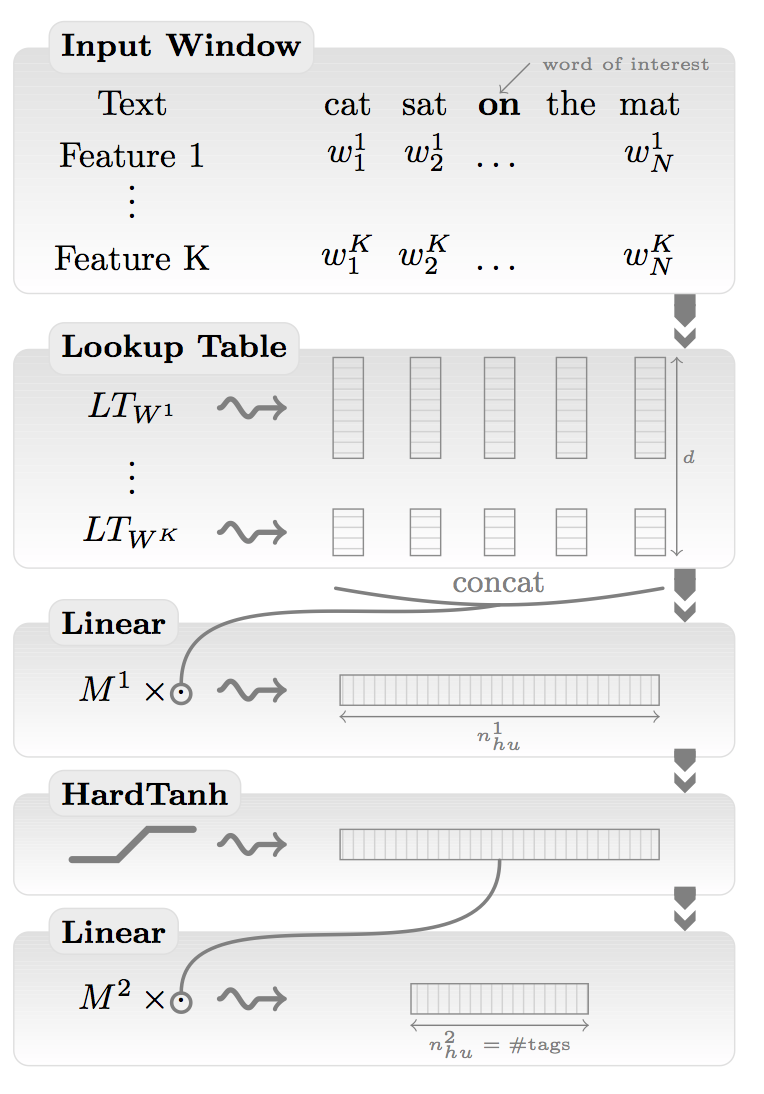
\includegraphics[scale=0.5]{../NLP-standalone-images/network.png}
\end{figure}

\subsubsection{Window approach}

We used a window that focuses on the word to classify. For example, if the sentence is "What is the birth date of the president of France?", and the word to classify is "date", for a window size of 7, the window is: "is the birth \textbf{date} of the president".

We used this window because neural networks works with a fixed number of input parameters. 
The window size is a meta parameter to choose. This window has to be large enough that we can decide in the context of the window in which category a word is. We used a window of size 7.

\subsubsection{Look up table}

The look up table is a dictionary that associates to each word $w$ a vector $V_w \in \mathbb{R}^n$, where n is the number of parameters we used to encode a word. We used $n=25$.
If two English words $w_1$ and $w_2$ are synonymous, then $||w_1-w_2||_2$ is small.

The construction of look-up table is described in \cite{collobert} and used unsupervised machine learning techniques.
We used a precomputed look up table, found here: \url{http://metaoptimize.com/projects/wordreprs/}

We also add one parameter that give us if the word starts with a capitalize character or not. Finally words are embedded in vectors of dimension 26. 

\subsubsection{The neural network}

We tried two different architectures:
-A linear model, i.e. without any hidden layers. This gives us $26\times 7\times 4 = 728$ parameters to optimize. 
-A non linear model with one hidden layer of size 10. This gives us $26\times 7\times 10\times 4 = 7280$ parameters to optimize.

The linear model has the advantage to have few parameters, so it can be learned with a small data set of annotated questions. However we found that this model is not enough powerful to catch the complexity of the problem we want to solve.
The non linear model is more complex and can describe with more precision how the English language works. But because of the huge number of parameters to learn, we need a larger annotated data set that we currently have.

We add one regularization parameter to limit over-training.
The neural network is implemented in Lua with the Torch7 framework.
Few minutes of computation are needed to train successfully the model.

\subsection{Results}

This baseline algorithm, witch was the goal for the midterm, give us quite good results.
The linear model has an accuracy of 80\% on the training set, and the non linear model has an accuracy of 98\% on the training set.
On the test set, these two models have an accuracy of 60\%, witch is much better than chance (a random method would give us 25\% of accuracy), but it is not efficient enough to be used for tricky questions (e.g. that are not closed to one of the sentence in our annotated data set).

\subsection{Future work}

\subsubsection{Unsupervised deep learning}

We could use auto-encoders  with Restrictive Boltzmann Machine (R.B.M) and an unsupervised data set of questions to learn a much more efficient representation of a question, as explained in \cite{fischer2012introduction} and in \cite{hinton2006reducing}

We can easily found large data set of non annotated questions.
One advantage of doing this is to limit supervision (because our annotated data set is very small), and it should improve the capacity of our model to generalize to questions that are not in our data set.

\subsubsection{Used a more efficient preprocessing}

We could reuse a part of the work done in the grammatical approach to have a better input for the neural network. For example, we could use the "Merge quotation nodes" and the "Merge named entities" steps to simplify input questions.

\subsubsection{Merge the work done with the grammatical approach}

This ML approach gives us, for each word of the sentence, the probability to be in the \textit{subject}, in the \textit{predicate}, in the \textit{object} or a word to ignore.
Maybe we can use this information to improve the accuracy of the grammatical approach.


